\chapter{Introduction}

\section{Exciting astrophysics happen far, far away}

We live in a boring part of the Universe. This allows life and the life sciences to thrive here. However, everything that is interesting in astrophysics takes place far, far away. For example, most \gls{grbs} take place about 1 Gpc \ref{anita2} away from us. That is over three billion light years away! 



\begin{figure}
\centering
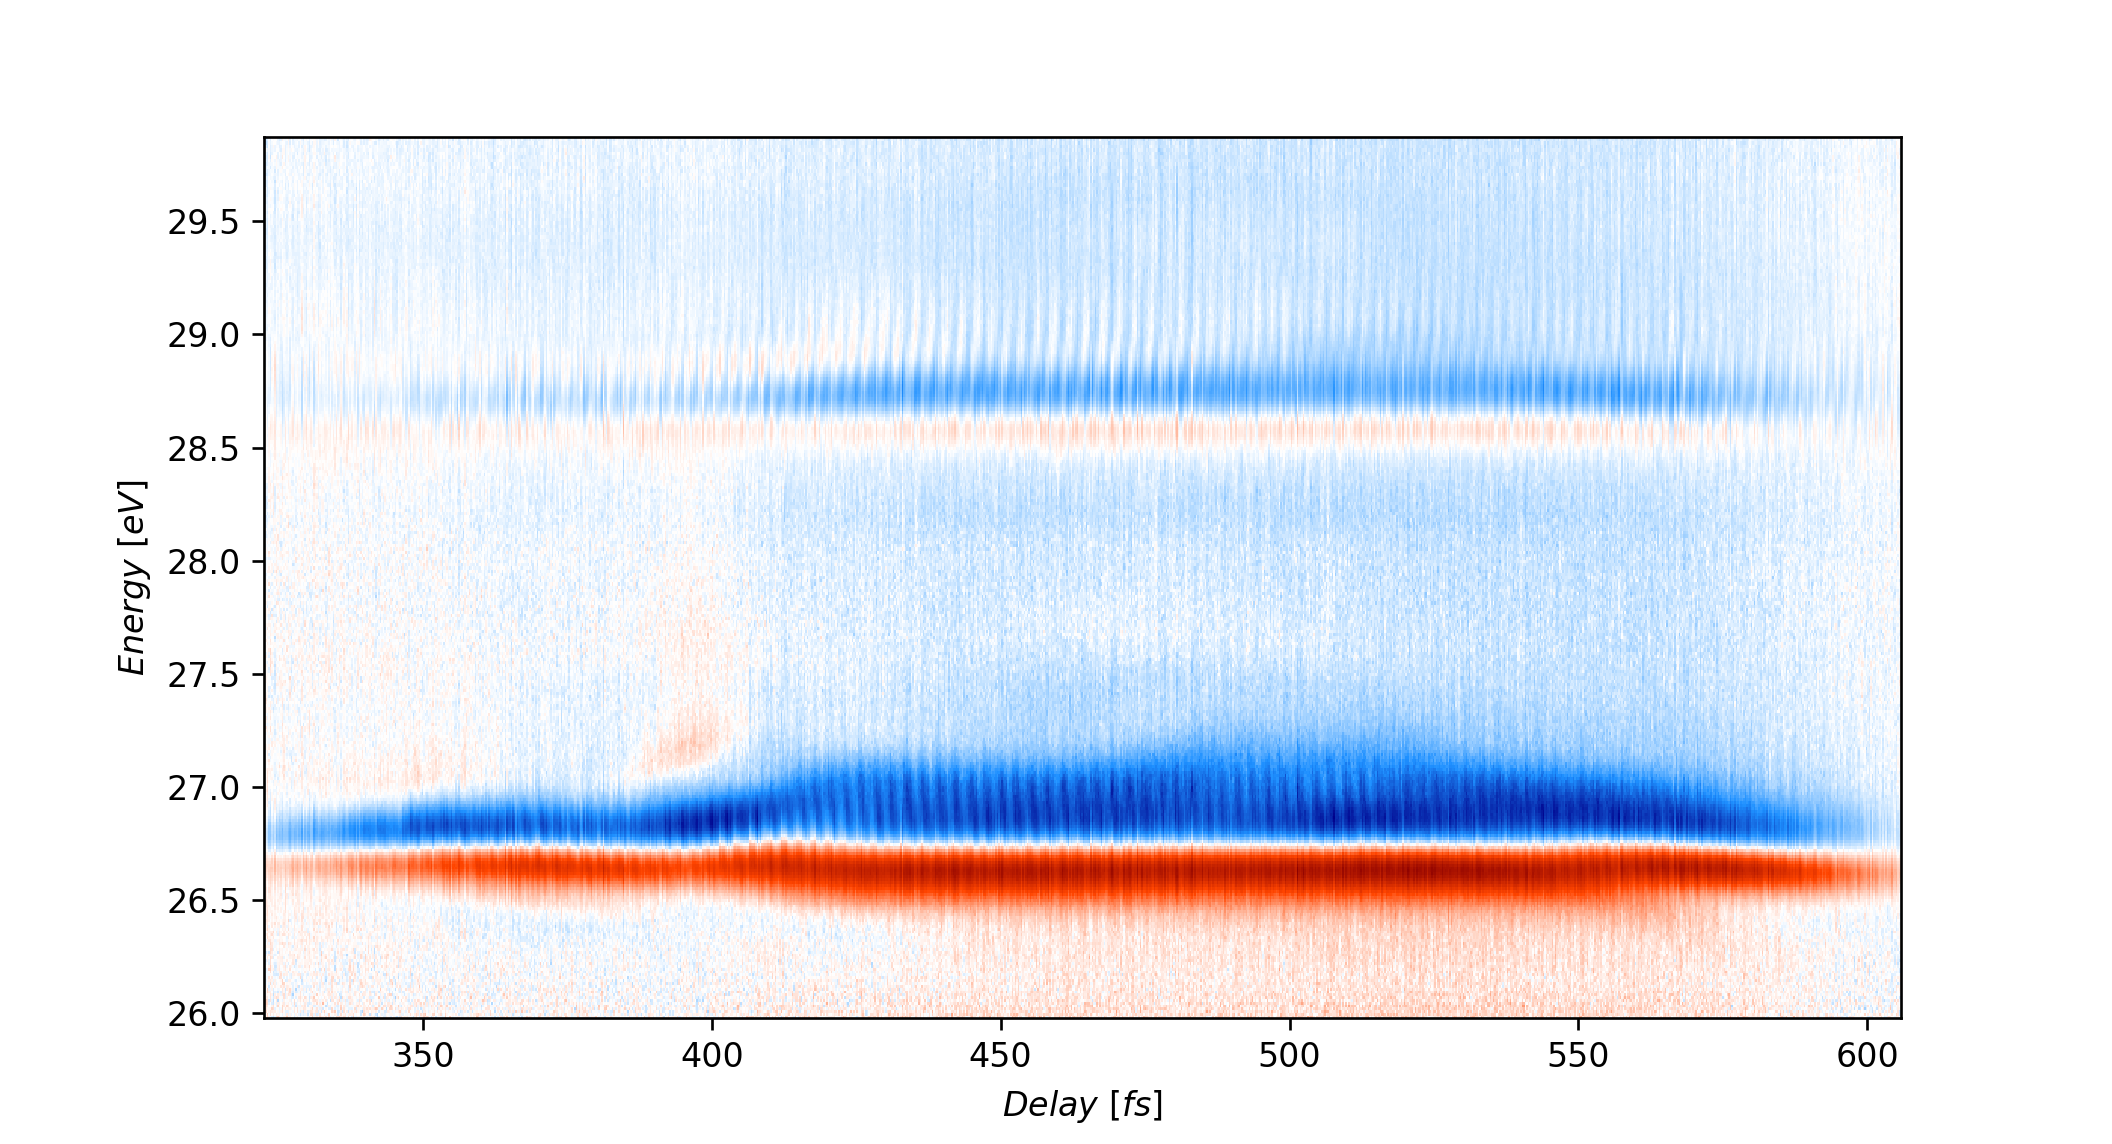
\includegraphics[width=0.5\textwidth]{figures/Introduction/6_forthesis.png}
\caption{Depiction of a GRB. Picture Credit: NASA E/PO, Sonoma State University, Aurore Simonnet.}
\label{grb}
\end{figure}

\section{Astrophysical messengers}

Traditional astrophysical messengers are not able to completely probe physics that take place at the farthest distances and at the highest energies. Since the beginning of astronomy, we have relied on optical light to study objects in the sky. In the last few decades, we have started utilizing light of other wavelengths such as X-rays and gamma rays. However, light of energy 1~MeV and above can undergo pair production. Light of energy 13.6~eV gets absorbed by Hydrogen atoms, the most abundant element in the Universe, while light at other wavelengths gets absorbed by other atoms and molecules. Light is the astronomer's best friend, but there is an inevitable need for complementary messengers.

Fortunately, in the last century, we have opened up multiple new windows t

%\begin{figure}
%\centering
%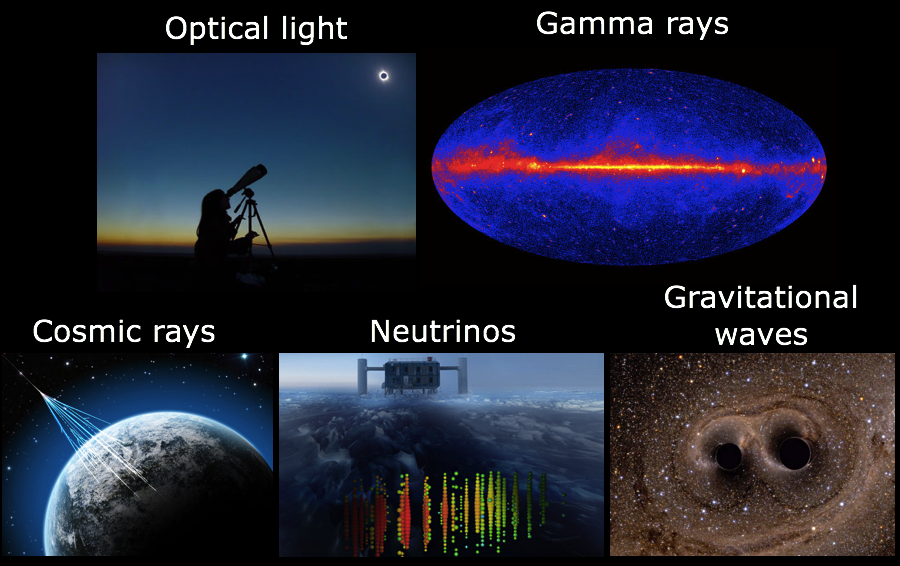
\includegraphics[width=1.0\textwidth]{figures/messengers.png}
%\caption{Astrophysical messengers. Pictures are all borrowed from Fermi, IceCube and LIGO collaborations, and the Internet.}
%\label{messengers}
%\end{figure}

\begin{figure}
\centering
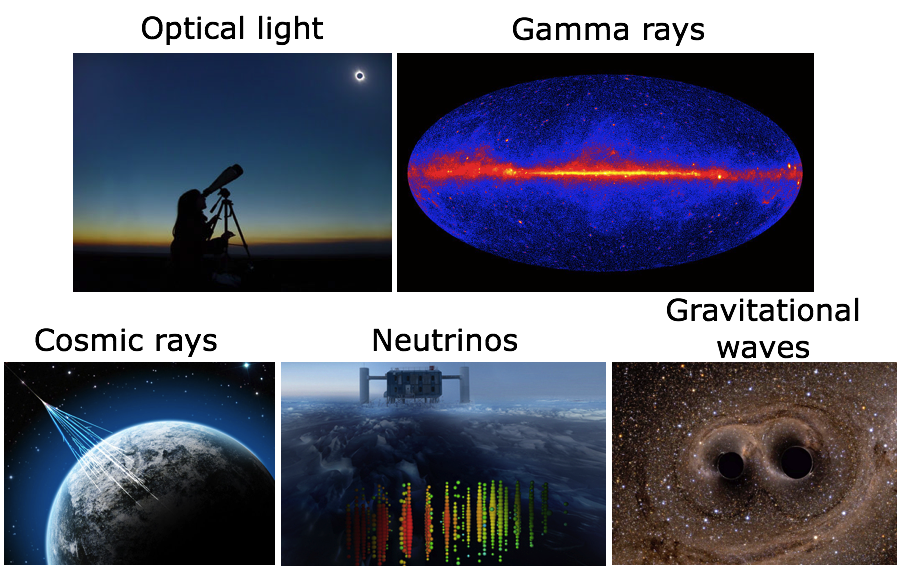
\includegraphics[width=1.0\textwidth]{figures/messengers_2.png}
\caption{Astrophysical messengers. Pictures are all borrowed from Fermi, IceCube and LIGO collaborations, and the Internet.}
\label{messengers}
\end{figure}

\section{Neutrinos as astrophysical messengers}

Neutrinos are potentially perfect candidates for carrying information about distant particle accelerators all the way to us. Due to being neutral and weakly interacting, neutrinos would remain unattenuated and point straight back to their source. In this way, they would have a definite advantage over messengers such as cosmic rays. Neutrinos are the side product of almost every nuclear reaction and can carry versatile information about particle physics taking place at cosmic distances. Their  

\begin{figure}
\centering
\subfloat[t]{
	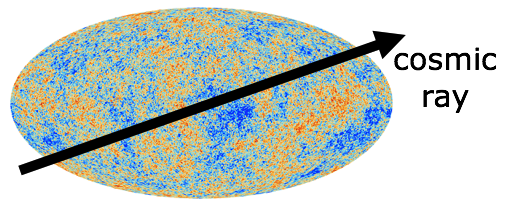
\includegraphics[width=0.8\textwidth, valign=c]	{figures/cosmogenic_2.png}
    \label{cosmogenic}
    }\quad
\subfloat[b]{
	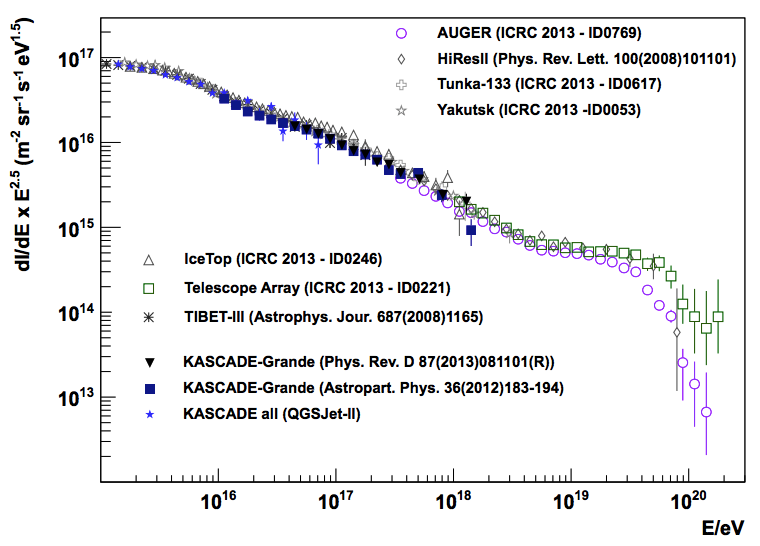
\includegraphics[width=0.8\textwidth, valign=c]{figures/kneeankle.png}
    \label{kneeankle}
    }
\caption{Top: Depiction of a cosmic ray interacting with the CMB. Thanks to the Planck telescope for the CMB picture. Bottom: Energy spectra of cosmic rays measured by different experiments. Andreas Haungs showed this plot at the 13th International Conference on Topics in Astroparticle and Underground Physics. UHE cosmic rays can only travel for about 50 Mpc before they interact with CMB photons and lose energy, therefore, we see a sharply falling spectrum at about $10^{20}\,\mbox{eV}$ energy.}
\label{cr}
\end{figure}

\begin{figure}
\centering
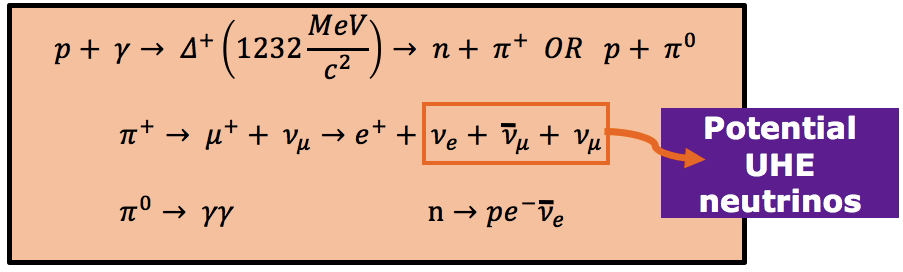
\includegraphics[width=1.0\textwidth]{figures/uhe_process.png}
\caption{A process for production of UHE neutrinos.}
\label{uhe_process}
\end{figure}

\section{Optical Cherenkov neutrino detectors}


IceCube and ANTARES are both optimized for the detection of muons from charged current interactions of high energy astrophysical neutrinos. IceCube uses the Antarctic ice as a target medium for high energy neutrinos to interact in. ANTARES uses sea-water instead. They both look for optical Cherenkov signatures of high energy neutrino interactions. ANTARES is sensitive to neutrinos of energy 10 GeV - 100 TeV. IceCube was built ceCube can also detect neutrinos of energy of order MeV. 


\begin{figure}
\centering
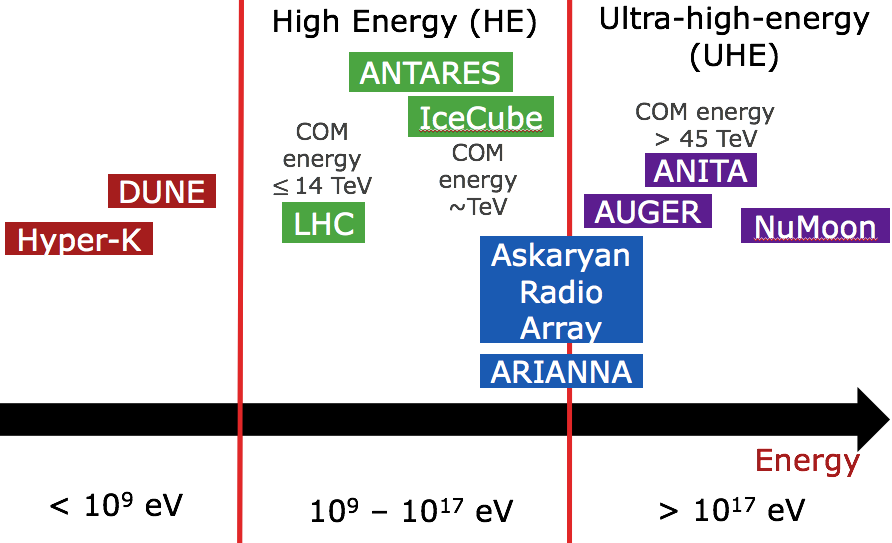
\includegraphics[width=0.9\textwidth]{figures/anita_where_energy.png}
\caption{The ANITA experiment looks for particles, specifically, neutrinos of energies that are to close to the extreme right of the energy scale.}
\label{anita_energy}
\end{figure}


\section{Radio Cherenkov neutrino detectors}

Radio Cherenkov neutrino experiments look for \gls{uhe} neutrinos in the energy regime of $> 10^{16}\,\mathrm{eV}$. The main challenge for detection by these experiments and a potential solution for detection are presented below. We also introduce two complementary radio Cherenkov experiments,andin this section. Where they are on the energy scale as compared to other particle physics experiments is shown in Figure



\subsection{Askaryan Effect}

f light in the medium. The particle shower would mainly consist of photons, electrons and positrons. As it travels through the dielectric, the particle shower develops about a 20\% negative charge. This happens primarily due to Compton scattering of electrons in the medium (so electrons leaving the medium and joining the shower) and secondarily due to annihilation of positrons in the shower with electrons in the medium (so positrons leaving the shower).   
As this charged particle shower travels through the medium at a speed greater than the speed of light in the medium, Cherenkov radiation is produced. If this Cherenkov radiation is observed at wavelengths larger than the shower's transverse dimension of about 10 cm, then it would be seen as coherent waves in radio frequencies. 

\begin{figure}
\centering
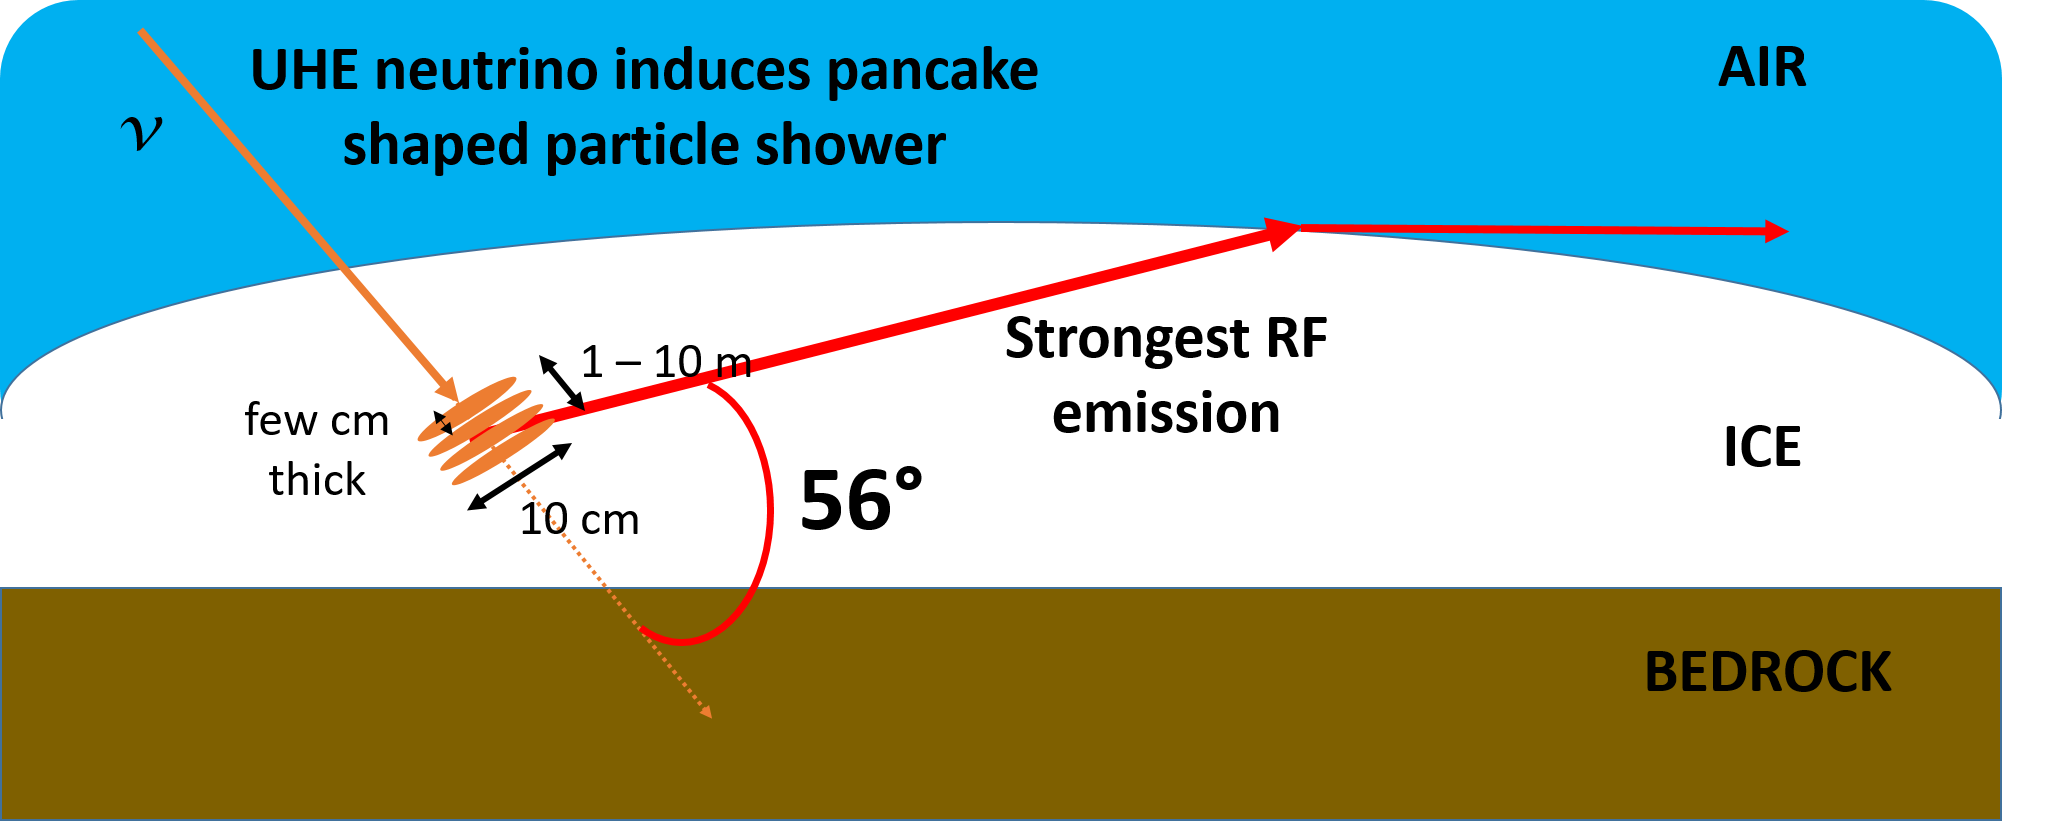
\includegraphics[width=1.0\textwidth]{figures/askaryan_in_ice.png}
\caption{A UHE neutrino could start a pancake-shaped particle shower in the ice.
Cherenkov radiation due to this particle shower would be coherent at wavelengths 
greater than the shower size of $\sim~10\,\mbox{cm}$, which correspond to radio waves.}
\label{askaryan}
\end{figure}

%ANITA and ARA use radio techniques to look for high energy neutrinos on the higher end of the energy spectrum as shown in Figure~\ref{anita_energy}. ARA covers the energy range $10^{16} - 10^{19}\, \mathrm{eV}$ which includes part of the UHE region and ANITA covers the UHE region from $10^{18}\, \mathrm{eV}$ and above. Below we provide a brief overview of these different experiments and how they complement one another.

\subsection{ANITA}

fect utilizing the Antarctic ice as the necessary dielectric target medium for neutrino interaction. Where \gls{anita}'s sensitivity lies in the energy scale as compared to other experiments in particle physics and particle astrophysics is presented in Figure=. A cartoon of an]oats up to an altitude of about 40 km and utilizes the polar vortex to fly in roughly circular orbits over the continent of Antarctica. At its float altitude, the balloon, upon gradual inflation, is bigger than the Ohio Stadium. There have been four flights of \gls{anita} so far. These are summarized in Figure

\begin{figure}
\centering
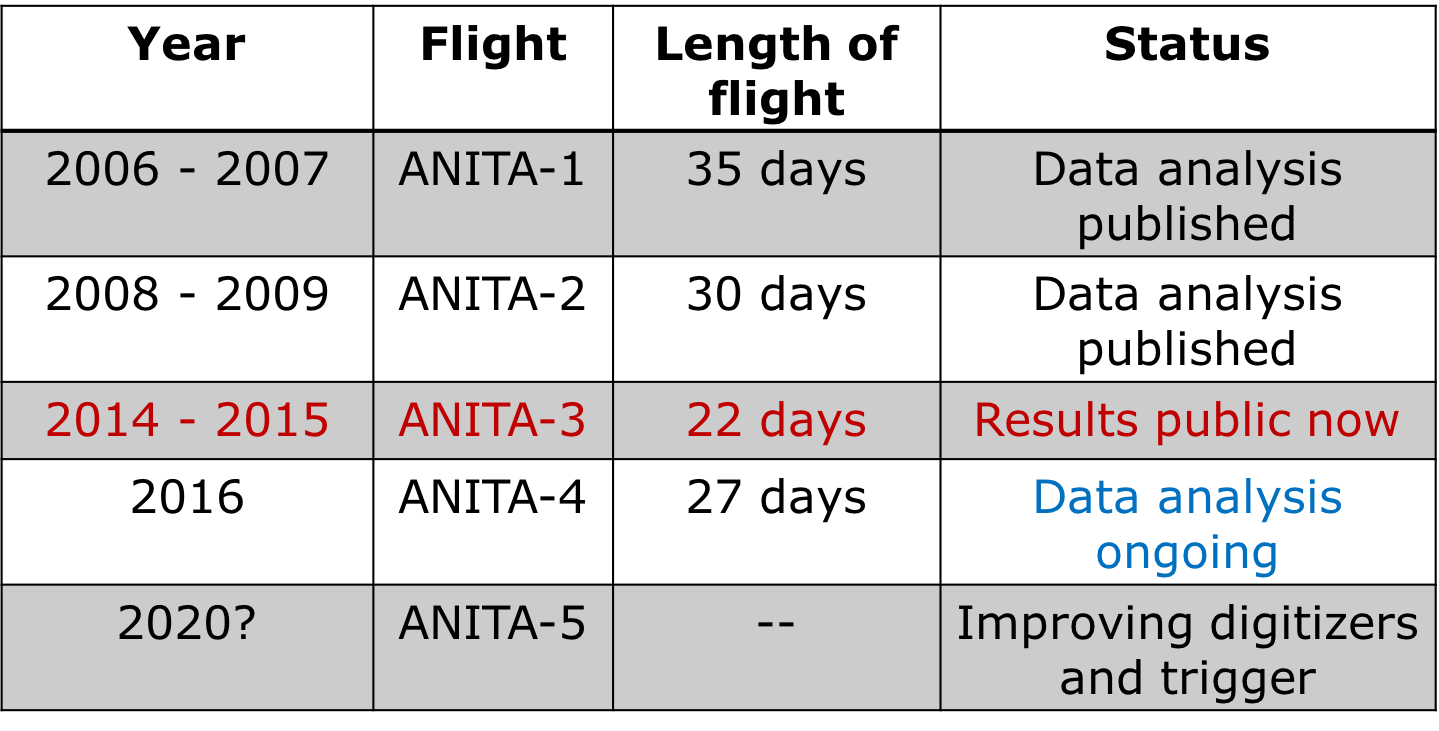
\includegraphics[width=1.0\textwidth]{figures/flights_table.png}
\caption{Summary of ANITA flights.}
\label{flights_summary}
\end{figure}


\begin{figure}
\centering
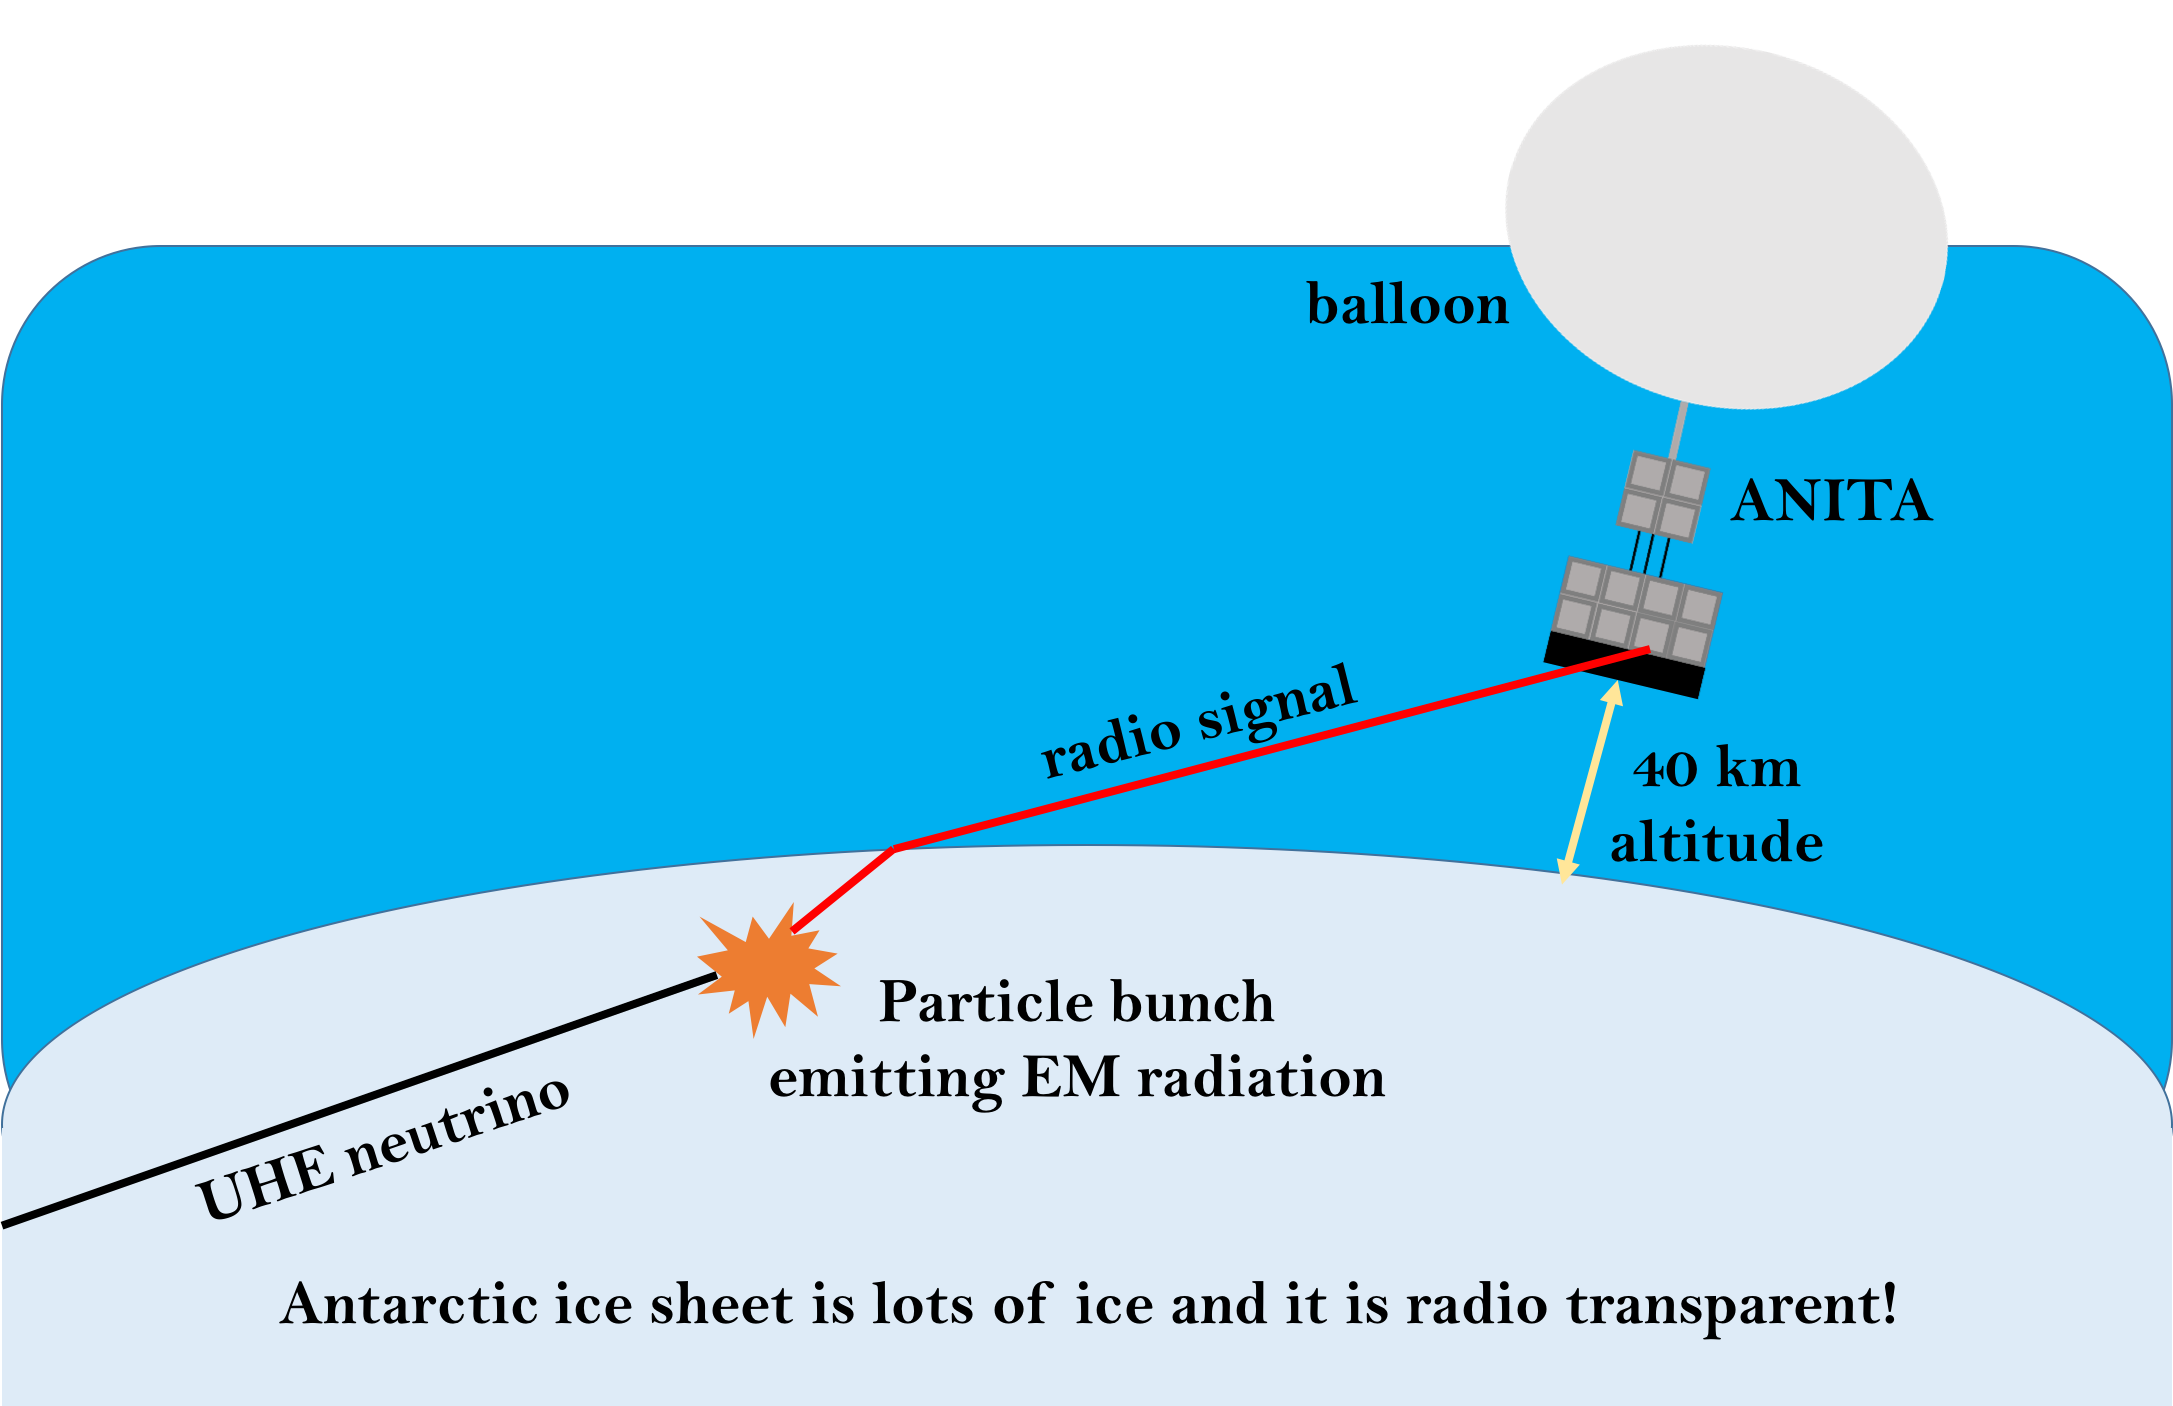
\includegraphics[width=0.9\textwidth]{figures/anita_cartoon_updated.png}
\caption{Concept of detection of UHE neutrinos with ANITA.}
\label{anita_cartoon}
\end{figure}

